\documentclass[12pt,a4]{article}
\usepackage[]{graphicx}\usepackage[]{xcolor}
% maxwidth is the original width if it is less than linewidth
% otherwise use linewidth (to make sure the graphics do not exceed the margin)
\makeatletter
\def\maxwidth{ %
  \ifdim\Gin@nat@width>\linewidth
    \linewidth
  \else
    \Gin@nat@width
  \fi
}
\makeatother

\definecolor{fgcolor}{rgb}{0.345, 0.345, 0.345}
\newcommand{\hlnum}[1]{\textcolor[rgb]{0.686,0.059,0.569}{#1}}%
\newcommand{\hlstr}[1]{\textcolor[rgb]{0.192,0.494,0.8}{#1}}%
\newcommand{\hlcom}[1]{\textcolor[rgb]{0.678,0.584,0.686}{\textit{#1}}}%
\newcommand{\hlopt}[1]{\textcolor[rgb]{0,0,0}{#1}}%
\newcommand{\hlstd}[1]{\textcolor[rgb]{0.345,0.345,0.345}{#1}}%
\newcommand{\hlkwa}[1]{\textcolor[rgb]{0.161,0.373,0.58}{\textbf{#1}}}%
\newcommand{\hlkwb}[1]{\textcolor[rgb]{0.69,0.353,0.396}{#1}}%
\newcommand{\hlkwc}[1]{\textcolor[rgb]{0.333,0.667,0.333}{#1}}%
\newcommand{\hlkwd}[1]{\textcolor[rgb]{0.737,0.353,0.396}{\textbf{#1}}}%
\let\hlipl\hlkwb

\usepackage{framed}
\makeatletter
\newenvironment{kframe}{%
 \def\at@end@of@kframe{}%
 \ifinner\ifhmode%
  \def\at@end@of@kframe{\end{minipage}}%
  \begin{minipage}{\columnwidth}%
 \fi\fi%
 \def\FrameCommand##1{\hskip\@totalleftmargin \hskip-\fboxsep
 \colorbox{shadecolor}{##1}\hskip-\fboxsep
     % There is no \\@totalrightmargin, so:
     \hskip-\linewidth \hskip-\@totalleftmargin \hskip\columnwidth}%
 \MakeFramed {\advance\hsize-\width
   \@totalleftmargin\z@ \linewidth\hsize
   \@setminipage}}%
 {\par\unskip\endMakeFramed%
 \at@end@of@kframe}
\makeatother

\definecolor{shadecolor}{rgb}{.97, .97, .97}
\definecolor{messagecolor}{rgb}{0, 0, 0}
\definecolor{warningcolor}{rgb}{1, 0, 1}
\definecolor{errorcolor}{rgb}{1, 0, 0}
\newenvironment{knitrout}{}{} % an empty environment to be redefined in TeX

\usepackage{alltt}
\newcommand{\SweaveOpts}[1]{}  % do not interfere with LaTeX
\newcommand{\SweaveInput}[1]{} % because they are not real TeX commands
\newcommand{\Sexpr}[1]{}       % will only be parsed by R



% ---- Metadata ---- %

\title{Honesty by Convenience: Corruption Tolerance in Ecuador}
\author{Daniel Sánchez}
\date{June 2022}

% ---- Load Packages ---- %

% Math

\usepackage{savesym} % Need to "save" the command that is already defined \varTheta

\usepackage{amsmath}
  \savesymbol{varTheta} 

% Fonts

% To set the TNR font for both text and equations:

\usepackage{mathspec}
  \setallmainfonts(Digits,Greek,Latin){Times New Roman}
\restoresymbol{MTP}{varTheta}

% Formatting

\usepackage{setspace}
  \doublespacing

\usepackage[margin = 1in]{geometry}

\usepackage{lscape}

% Setting the size of the section titles

\usepackage{titlesec}

\titleformat*{\section}{\normalsize\bfseries}

% Citation & Bibliographies

\usepackage[backend = biber, style = apa, citestyle = apa]{biblatex}
  \addbibresource{refs.bib}
  
% For tables:

 % For the modelsummary tables:
\usepackage{siunitx}
\usepackage{booktabs} 
  \newcolumntype{d}{S[input-symbols = ()]}
\usepackage{multirow}
\usepackage[flushleft]{threeparttable}

% For figure and table captions

\usepackage{caption}
  \captionsetup{labelfont = bf} % All in bold  
  
% Other packages

\usepackage{csquotes} % For quotation marks

\usepackage{epigraph} % For epigraph
  \setlength\epigraphwidth{9cm}
  \setlength\epigraphrule{1pt}

\usepackage{float} % For the H float option- only used in emergencies (lol)

\usepackage{textcomp} % For the registered trademark symbol.

% Always load these packages at the end of the preamble:

\usepackage{hyperref}

% ---- R Stuff to be used in the whole document ----

% Here I will execute or source R code through chunks that I need to use throughout the whole document.

% General settings



% Load the data by sourcing the data manipulation script. Note that survey design objects are indeed created in this script.
% We use the time argument in the chunks to reread or rerun the chunk in case external files are updated and chunks need to be rerun and re-cached.


% Perform all survey-robust tabulations by sourcing the R Script. 
% These are used on the text later.


% Run the first models




\begin{document}
% Results II .Rnw File

\section{Results}
\label{sec:results}
Section \ref{sec:background} identified some key events which happenned at the same time of the corruption tolerance increase. Two economic variables observed at the individual level through the AB significantly changed during this period: the percent of people who report a worse economic situation as well as unemployment. Variables which proxy attitudes in the political landscape have also significantly changed: the percentage of people who confide in the President, the percentage who approve the President's job and also the percentage of people who identify with the political right wing. These variables where used for simple empirical models, which follow the equation below.

\begin{equation}
\label{eqn:simplemod}
P(ctol = 1 | \textbf{\textit{X}} \hspace{0.04cm}) = G \left[ \beta_0 + \delta_0 y_{16} + \beta_1 x^* + \delta_1 (y_{16} \cdot x^*)\right]
\end{equation}
where the key regressor $x^*$ can be: a dummy variable set to unity for respondents who answered that their economic situation is worse (Model 1), a dummy variable set to unity for those who report being unemployed (Model 2), a discrete variable with numbers 1-7, where higher values imply a higher degree of confidence in the President (Model 3), a discrete variable with numbers 1-5, with higher numbers implying a higher rating of the President's job performance (Model 4) or a discrete variable with numbers from 1-10 where 1 is the extreme left and 10 is the extreme right (Model 5). 

Table \ref{tab:simplemodel} presents coefficients of the logistic model for Equation \ref{eqn:simplemod} and Table \ref{tab:apesimp} presents their associated average partial effects. It is show that an unemployed person is 5.9\% more likely to justify corruption. Additionally, a respondent who answered one number higher for an increased degree of confidence in the President was 2.4\% less likely to justify corruption. Finally, a person who rated the President's job performance one unit higher was 4.4\% less likely to justify corruption. All other partial effects are not significant.

% Now, I'll make the table with modelsummary from the sourced stuff. 
\begin{table}[htbp]
\caption{Logit coefficients for baseline models}
\label{tab:simplemodel}

\begin{tabular}[t]{lccccc}
\toprule
  & Model 1 & Model 2 & Model 3 & Model 4 & Model 5\\
\midrule
Constant & \num{-1.894}*** & \num{-1.989}*** & \num{-0.455}** & \num{0.553} & \num{-1.527}***\\
 & (\num{0.127}) & (\num{0.110}) & (\num{0.208}) & (\num{0.362}) & (\num{0.196})\\
2016 Dummy & \num{0.848}*** & \num{1.001}*** & \num{-0.188} & \num{-1.251}*** & \num{0.278}\\
 & (\num{0.158}) & (\num{0.132}) & (\num{0.238}) & (\num{0.415}) & (\num{0.234})\\
Worse Economic Situation & \num{0.131} &  &  &  & \\
 & (\num{0.169}) &  &  &  & \\
Unemployment &  & \num{1.015}*** &  &  & \\
 &  & (\num{0.205}) &  &  & \\
Confidence in President &  &  & \num{-0.288}*** &  & \\
 &  &  & (\num{0.037}) &  & \\
Approval of Pres. Performance &  &  &  & \num{-0.648}*** & \\
 &  &  &  & (\num{0.096}) & \\
Political Wing &  &  &  &  & \num{-0.047}\\
 &  &  &  &  & (\num{0.038})\\
Econ. Situation Interaction & \num{-0.025} &  &  &  & \\
 & (\num{0.197}) &  &  &  & \\
Unemployment Interaction &  & \num{-1.005}*** &  &  & \\
 &  & (\num{0.256}) &  &  & \\
Pres. Confidence Interaction &  &  & \num{0.206}*** &  & \\
 &  &  & (\num{0.044}) &  & \\
Pres. Approval Interaction &  &  &  & \num{0.568}*** & \\
 &  &  &  & (\num{0.111}) & \\
Pol. Wing Interaction &  &  &  &  & \num{0.095}**\\
 &  &  &  &  & (\num{0.043})\\
\midrule
$N$ & \num{2948} & \num{2950} & \num{2944} & \num{2941} & \num{2535}\\
AIC & \num{2893.64} & \num{2889.04} & \num{2848.57} & \num{2844.82} & \num{2574.81}\\
BIC & \num{2926.37} & \num{2920.98} & \num{2881.80} & \num{2876.65} & \num{2606.10}\\
\bottomrule
\end{tabular}


\vspace{0.25cm}
Logit coefficients of baseline models (Equation \ref{eqn:simplemod}) with design-adjusted std. errors.\\
*$p$ < 0.1, **$p$< 0.05, ***$p$ < 0.01.
\end{table}

% Do the APE table
\begin{table}[htbp]
\caption{Average partial effects for logit models in Table \ref{tab:simplemodel}}
\label{tab:apesimp}

\begin{tabular}[t]{lccccc}
\toprule
  & Model 1 & Model 2 & Model 3 & Model 4 & Model 5\\
\midrule
2016 Dummy & \num{0.131}*** & \num{0.126}*** & \num{0.109}*** & \num{0.117}*** & \num{0.124}***\\
 & (\num{0.020}) & (\num{0.019}) & (\num{0.019}) & (\num{0.019}) & (\num{0.020})\\
Worse Economic Situation & \num{0.018} &  &  &  & \\
 & (\num{0.014}) &  &  &  & \\
Unemployment &  & \num{0.058}*** &  &  & \\
 &  & (\num{0.020}) &  &  & \\
Confidence in President &  &  & \num{-0.024}*** &  & \\
 &  &  & (\num{0.003}) &  & \\
Approval of Pres. Performance &  &  &  & \num{-0.044}*** & \\
 &  &  &  & (\num{0.008}) & \\
Political Wing &  &  &  &  & \num{0.003}\\
 &  &  &  &  & (\num{0.003})\\
\midrule
$N$ & \num{2948} & \num{2950} & \num{2944} & \num{2941} & \num{2535}\\
\bottomrule
\end{tabular}


\vspace{0.25cm}
Average partial effects for models in Table \ref{tab:simplemodel}, with design-adjusted std. errors.\\
*$p$ < 0.1, **$p$< 0.05, ***$p$ < 0.01.
\end{table}

Consider the logit coefficients in Table \ref{tab:simplemodel}. The coefficient for the year dummy confirms the significance of the corruption tolerance increase in 2016, which is lost when considering interaction terms with confidence in the President, and actually has a negative sign with the other political variables. The inclusion of unemployment and economic situation do not eliminate the significance of the year dummy. Model 1 suggests that a person who reports having a worse economic situation does not tolerate corruption differently than those who report a same or equal economic situation. According to Model 2, respondents who were unemployed were more likely to justify corruption than those who were not unemployed\footnote{In this case, not being unemployed means either being employed, salary and hours worked notwithstanding, and also not being in the labor force (students, rentists, among others). Results all throughout this paper are robust to including an employment variable.} The interaction term in this model has a negative sign, which shows that the effect of unemployment in 2016 was less than the effect in 2014, meaning unemployed people actually justified corruption less after political instability set in. 

Models 3 and 4 display the same relationship: people who either trust or approve of the President in a higher degree also tolerate corruption less. A more zealous supporter of the regime believed bribes were not justified; however, this appears to change for 2016. The interaction terms for both variables are significant and positive: in 2016 supporters started to justify corruption more. This could explain the jump in corruption tolerance as regime support eroded in 2016, which meant that the number of non-supporters was higher and these respondents justified corruption more than supporters. Also, the supporters that remained started to justify bribes to a higher degree. In Model 3, the significance of the year dummy is lost, while in Model 4 its sign reversed.

The coefficients in Model 5 show that a person who identifies closer to the political right does not justify corruption more or less relative to those identifying closer to the political left. However, the interaction term shows that people answering higher values of this variable justified corruption more in 2016. Once again, the significance of the year dummy is lost when considering this variable. With a higher number of respondents identifying with the political right wing, who appear to justify corruption more, it would be understood how overall corruption tolerance increased.

% I need to draw the graph which shows the visual differences between groups and their corruption tolerance

% Now I do the data wrangling needed for this


% Now do the graph
\begin{figure}[htbp]
\caption{Graphical representations of corruption tolerance across key explanatory variables}
\label{fig:difgraph}
\fbox{
\begin{minipage}{\textwidth}
\begin{knitrout}
\definecolor{shadecolor}{rgb}{0.969, 0.969, 0.969}\color{fgcolor}

{\centering 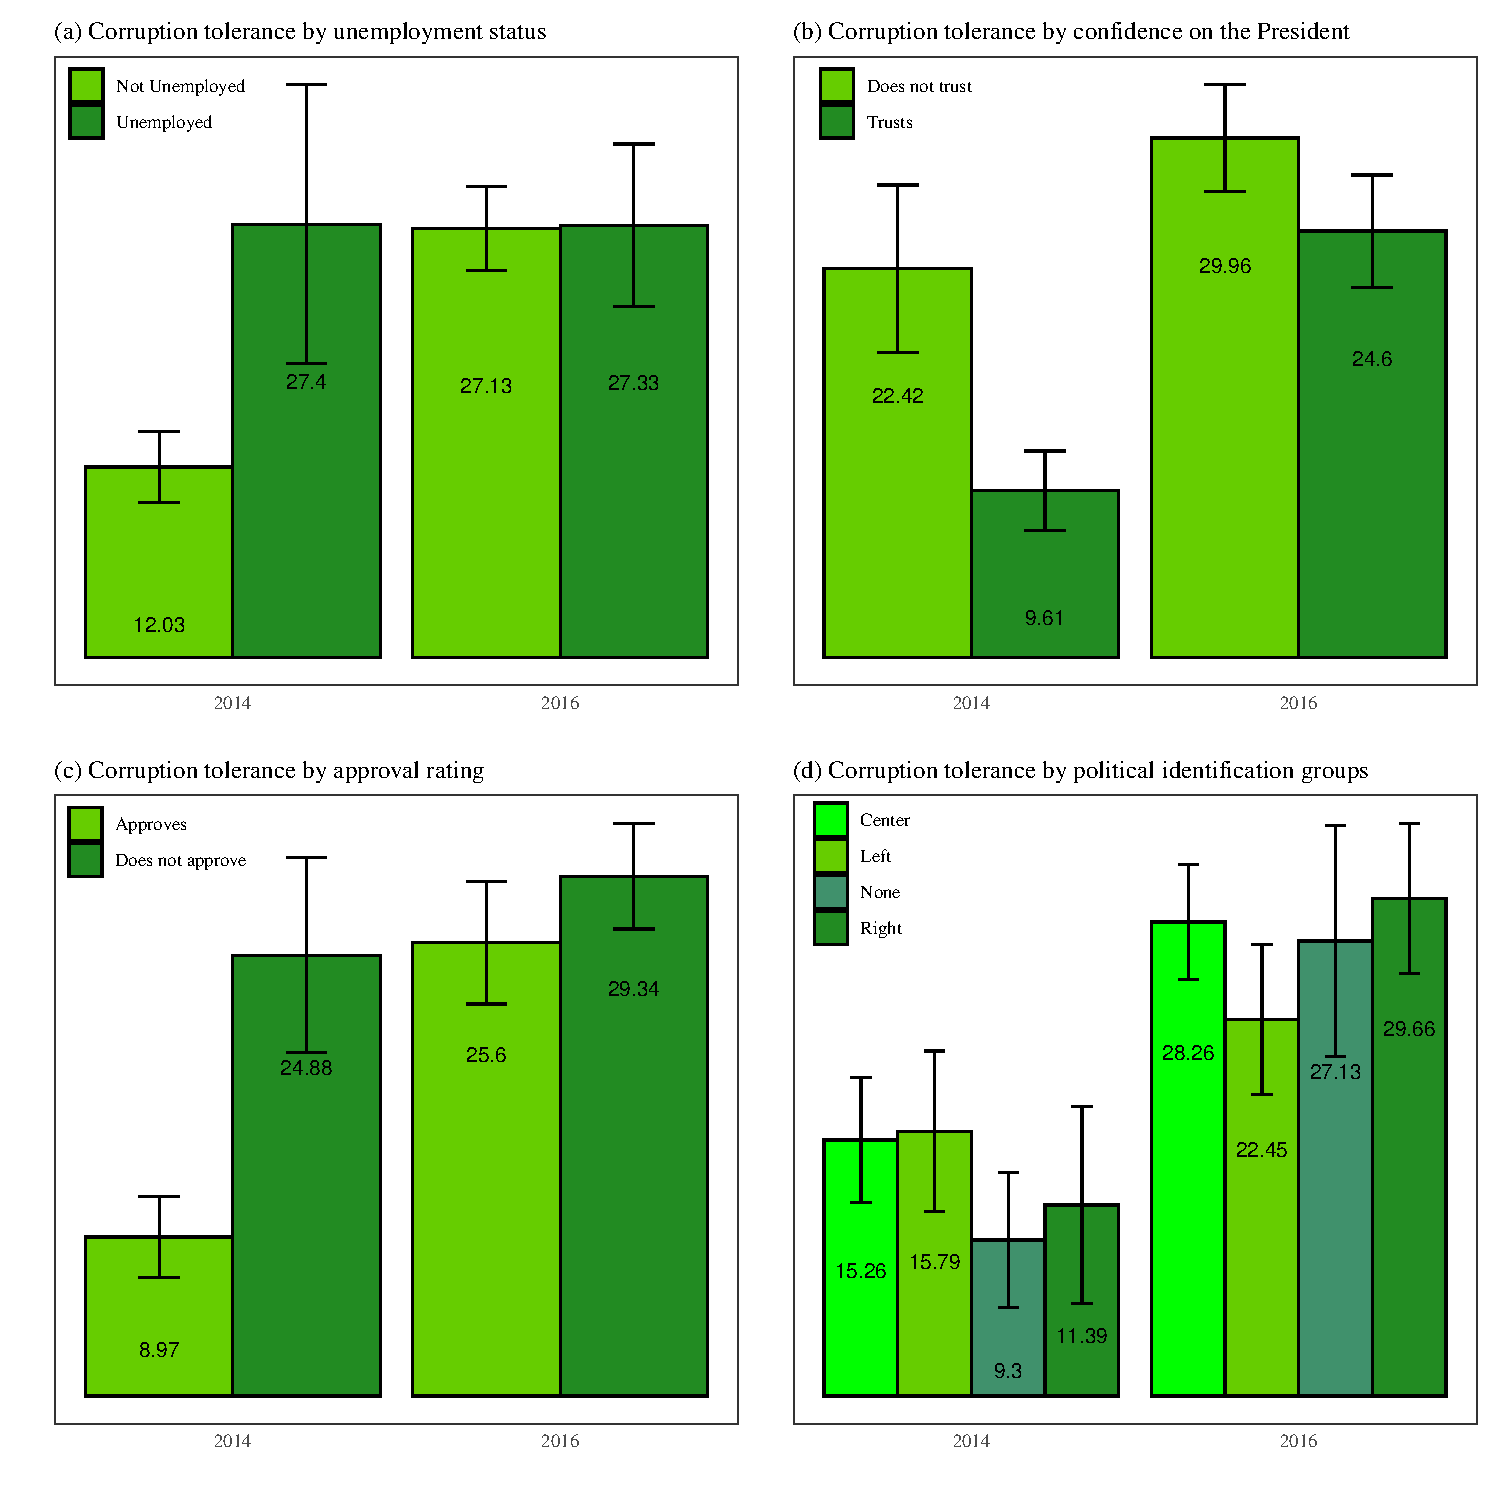
\includegraphics[width=\maxwidth]{figure/difgraph-1} 

}


\end{knitrout}
Figures show the percent of respondents that justify corruption across the groups used as explanatory models in Table \ref{tab:simplemodel}.Error bars represent the 95\% confidence intervals adjusted for design effects. 
\end{minipage}
}
\end{figure}

These findings are supported by Figure \ref{fig:difgraph}. According to panel (a), in 2014, only 12.03\% of those not unemployed justified corruption, while in 2016 this figure increased to 27.03\%, very close to the percentage of unemployed people who justified it in 2016. The time difference between these point estimates is not statistically significant, which means that in 2016 the effect of unemployment in corruption tolerance approached zero. Thus, Figure \ref{fig:difgraph} along with Model 2 of Table \ref{tab:simplemodel} show that it was not the unemployed who started to justify corruption less, it was that the people who were not unemployed started to justify it more. Panels (b) and (c) of Figure \ref{fig:difgraph} show that the percentage of people who either confided in or approved the President and justified corruption increased significantly  between 2014 and 2016. This means that the negative effect of supporting the executive in 2016 was smaller than in 2014, as confirmed by the interaction term in Models 3 and 4 of Table \ref{tab:simplemodel}. In panel (d) of Figure \ref{fig:difgraph}, where four different political groups are considered: the left, right, center and those who did not answer the question. All four groups saw increases in the percent of group members who justify corruption. All increases in corruption tolerance are significant, except for those who identify with the left wing. This is consistent with the coefficient sign seen in Model 5 for the political score variable. 

\end{document}
